% Drawing 83/03-2 -- folder 83, batch 03, archive page 52 (PDF page 53).
% Transcription: un pentagone avec son étoile de diagonales intérieures, en marge
% Kind: pentagon with interior strokes. Method 2 (schematic redraw from the facsimile). Status: ok.
% Notes: Pentagon, its five sides drawn between the same computed vertices (on the page the left side stops short of the left vertex and resumes below it; joined here). The second strokes doubling the lower left side and crossing the lower right side below the bottom vertex are drawn as on the page, as is the tail stroke leaving the lower left side towards the text at the bottom left. Inside there are only short broken strokes and dots, not full diagonals: they are drawn one by one where they stand. These fragments do not line up into the five diagonals, so the "star of diagonals" of the transcription is a reading that the redraw does not impose (perhaps an erased pencil star whose ink remains in pieces); the scribble at the far bottom left belongs to the text line and is left out. Redrawn 2026-11-09 (issue 128): to check again.
% Coordinates: 1 unit = 1 mm = 1/100 of the crop width (bbox in page fractions: [0.19, 0.39, 0.33, 0.47]).
% Redrawn by Claude (claude-opus-5-5), issue #73, 2026-11-09; not checked by a human; not compiled (no TeX in the session).
% Rights: reproduces part of the work -- behind RENDER_TRANSCRIPTS, never published by itself.
\documentclass[tikz,border=3pt]{standalone}
\usepackage{amsmath,amssymb}
\usetikzlibrary{patterns,arrows.meta}
\tikzset{pencil/.style={black!45}, struck/.style={black!35}, mark/.style={circle,draw,inner sep=1.3pt}, pt/.style={circle,fill,inner sep=0.9pt}, opt/.style={circle,draw,fill=white,inner sep=1.1pt}}
\begin{document}
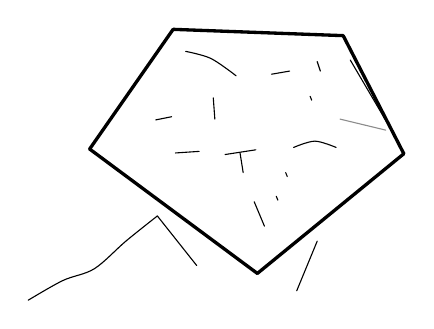
\begin{tikzpicture}[x=1mm,y=1mm,line cap=round,line join=round,font=\scriptsize]
\draw[very thick] (32,-23.6) -- (53.6,-24.4);
\draw[very thick] (53.6,-24.4) -- (61.3,-39.4);
\draw[very thick] (61.3,-39.4) -- (42.7,-54.6);
\draw[very thick] (42.7,-54.6) -- (21.4,-38.8);
\draw[very thick] (21.4,-38.8) -- (32,-23.6);
\draw (30,-47.3) -- (35,-53.6);
\draw (50.3,-50.5) -- (47.7,-56.8);
\draw (54.5,-27.5) -- (59.2,-35.5);
\draw plot[smooth, tension=0.55] coordinates {(30,-47.3) (26,-50.5) (22,-54) (18,-55.5) (13.6,-58)};
\draw plot[smooth, tension=0.55] coordinates {(33.6,-26.4) (36.8,-27.3) (40,-29.5)};
\draw (44.5,-29.3) -- (46.8,-28.9);
\draw (50.3,-27.7) -- (50.7,-28.9);
\draw (37.1,-32.3) -- (37.3,-35);
\draw (29.8,-35.1) -- (31.8,-34.7);
\draw[pencil] (53.2,-35) -- (59,-36.4);
\draw (32.3,-39.3) -- (35.3,-39.1);
\draw (38.6,-39.5) -- (42.5,-38.9);
\draw (40.5,-39.3) -- (40.9,-41.8);
\draw plot[smooth, tension=0.55] coordinates {(47.3,-38.6) (50,-37.8) (52.7,-38.6)};
\draw (42.3,-45.5) -- (43.6,-48.6);
\draw (49.4,-32.1) -- (49.6,-32.6);
\draw (46.3,-41.8) -- (46.5,-42.3);
\draw (45.1,-44.8) -- (45.3,-45.3);
\end{tikzpicture}
\end{document}
